\section{Groups}
    While monoids are structurally simpler than groups, the notion of a group
    is one of the most basic and fundamental algebraic structures that one can
    consider.
    \begin{fdefinition}{Group}{Group}
        A group is a \gls{monoid} $(G,*)$ such that for all $g\in{G}$, $g$ is
        an \gls{invertible element} with respect to $*$. That is:
        \index{Group}
        \begin{itemize}
            \setlength\itemsep{0em}
            \item The binary operation $*$ is associative.
            \item There exists a unital element $e\in{G}$.
            \item For every element $a\in{A}$, there is an inverse element.
        \end{itemize}
    \end{fdefinition}
    Note that it is not necessarily true that $a*b=b*a$. Such groups are called
    Abelian. There are several examples of groups that one is likely familiar
    with.
    \begin{example}
        If $+$ denotes the usual addition on $\mathbb{Z}$, then
        $(\mathbb{Z},+)$ is a group. The unital element is 0, and for all
        $n\in\mathbb{Z}$, $\minus{n}$ is an inverse element of $n$. That is,
        $n+(\minus{n})=0$, which is a unital element. Moreover, addition is
        associative and therefore $(\mathbb{Z},+)$ is a group.
    \end{example}
    \begin{example}
        If $\mathbb{R}^{+}$ denotes the positive real numbers, and if $\cdot$
        denotes the usual multiplication of real numbers, then
        $(\mathbb{R},\cdot)$ is a group. For this group, 1 is the unital
        element for all $r\in\mathbb{R}^{+}$, $1/r$ is the inverse element.
        Lastly, the operation is indeed associative.
    \end{example}
    \begin{example}
        Consider $\mathbb{Z}_{4}$ with it's modular addition $+$. Then
        $(\mathbb{Z}_{4},+)$ is a group. We can represent the operation $+$ with
        the following table:
        \begin{table}[H]
            \centering
            \captionsetup{type=table}
            \begin{tabular}{c|cccc}
                $+$&0&1&2&3\\
                \hline
                0&0&1&2&3\\
                1&1&2&3&0\\
                2&2&3&0&1\\
                3&3&0&1&2
            \end{tabular}
            \caption{The Group Structure of $\mathbb{Z}_{4}$}
        \end{table}
    \end{example}
    \begin{example}
        More generally, consider $\mathbb{Z}_{n}$ with modular addition $+$.
        Then $(\mathbb{Z}_{n},+)$ is a group. The unital element is $0$ since
        for all $k\in\mathbb{Z}_{n}$, $k+0=k$. The inverse of
        $k\in\mathbb{Z}_{n}$ is the unique integer $m\in\mathbb{Z}_{n}$ such
        that $k+m=n$. That is, $m=n-k$. For then $k+m=n$, and $n$ is equivalent
        to zero in $\mathbb{Z}_{n}$. Since modular addition is commutative, it
        follows that $0$ is a left and right unital element and that each
        element is left and right invertible, and thus $(\mathbb{Z}_{n},+)$ is a
        group.
    \end{example}
    \begin{theorem}
        If $G$ is a set, if $*$ is an associative binary operation on $G$, if
        $e\in{G}$ is a unique right unital element, and if for all $g\in{G}$ it
        is true that $g$ is weakly right invertible, then $G$ is a group.
    \end{theorem}
    \begin{proof}
        For by
        Thm.~\ref{thm:existence_of_weak_left_and_weak_right_implies_unital},
        $e$ is a unital element. And by
        Thm.~\ref{thm:unqiue_right_unit_and_weak_r_inv_implies_inv}, for all
        $g\in{G}$ it is true that $g$ is invertible. Therefore, $(G,*)$ is a
        group (Def.~\ref{def:Group}).
    \end{proof}
    Thus it suffices to check that there is a unique right identity and that all
    elements are weakly right intertible. The unital element of a group is
    unique (Thm.~\ref{thm:Unital_Elements_are_Unique}), as are the inverses of
    elements (Thm.~\ref{thm:Assoc_Op_Inverses_are_Unique}). Moreover, the
    inverse of a unital element is itself
    (Thm.~\ref{thm:Unital_Elements_Are_Invertible}).
    \begin{theorem}
        \label{thm:Group_Inverse_of_Product}%
        If $(G,*)$ is a group and $a,b\in G$, then:
        \begin{equation}
            (a*b)^{\minus{1}}=b^{\minus{1}}*a^{\minus{1}}
        \end{equation}
    \end{theorem}
    \begin{proof}
        For if $(G,*)$ is a group, and if $a,b\in{G}$, then $*$ is associative
        and $a$ and $b$ are invertible (Def.~\ref{def:Group}). But then by
        Thm.~\ref{thm:assoc_op_prod_of_inv_is_inv},
        $a*b=b^{\minus{1}}*a^{\minus{1}}$.
    \end{proof}
    \begin{theorem}
        \label{thm:Group_Inverse_of_Inverse}%
        If $(G,*)$ is a group and $a\in{G}$, then:
        \begin{equation}
            (a^{\minus{1}})^{\minus{1}}=a
        \end{equation}
    \end{theorem}
    \begin{proof}
        For if $e$ is the unital element of $G$, then:
        \begin{align}
            a^{\minus{1}}*(a^{\minus{1}})^{\minus{1}}
            &=(a^{\minus{1}}* a)^{\minus{1}}
            \tag{Thm.~\ref{thm:Group_Inverse_of_Product}}\\
            &=e
            \tag{Inverse Property}
        \end{align}
        From the uniqueness of inverses
        (Thm.~\ref{thm:Assoc_Op_Inverses_are_Unique}),
        $(a^{\minus{1}})^{\minus{1}}=a$.
    \end{proof}
    One of the fundamental aspects of elementary algebra is adding and
    subtracting like expressions from two sides of an equation. That is, if we
    are given $4x+1=9$, we solve this by adding $\minus{1}$ to both sides, and
    then dividing both sides by $4$ yielding $x=2$. Such procedures are valid
    because of the \textit{cancellation laws}\index{Cancellation Law} of real
    number arithmetic. These laws hold for groups, as well.
    \begin{ltheorem}{Left Cancellation Law}{Group_Left_Cancellation_Law}
        \index{Cancellation Law!Left}%
        If $(G,*)$ is a group, if $a,b,c\in{G}$, and if $a*b=a*c$, then $b=c$.
    \end{ltheorem}
    \begin{proof}
        For let $e$ be the unital element of $G$. Then:
        \par\vspace{-2.5ex}
        \begin{minipage}[t]{0.49\textwidth}
            \centering
            \begin{align}
                b&=e*b
                \tag{Identity}\\
                &=(a^{\minus{1}}*a)*b
                \tag{Inverse}\\
                &=a^{\minus{1}}*(a*b)
                \tag{Associativity}\\
                &=a^{\minus{1}}*(a*c)
                \tag{Hypothesis}
            \end{align}
        \end{minipage}
        \hfill
        \begin{minipage}[t]{0.49\textwidth}
            \centering
            \begin{align}
                &=(a^{\minus{1}}*a)*c
                \tag{Associativity}\\
                &=c*e
                \tag{Inverse}\\
                &=c
                \tag{Identity}
            \end{align}
        \end{minipage}
        \par\vspace{2.5ex}
        Thus by the transitivity of equality
        (Thm.~\ref{thm:Transitivity_of_Equality}), $b=c$.
    \end{proof}
    \begin{ltheorem}{Right Cancellation Law}{Group_Right_Cancellation_Law}
        \index{Cancellation Law!Right}%
        If $(G,*)$ is a group, if $a,b,c\in{G}$, and if $b*a=c*a$, then $b=c$.
    \end{ltheorem}
    \begin{proof}
        For let $e$ be the unital element of $G$. Then:
        \par\vspace{-2.5ex}
        \begin{minipage}[t]{0.49\textwidth}
            \centering
            \begin{align}
                b&=b*e
                \tag{Identity}\\
                &=b*(a*a^{\minus{1}})
                \tag{Inverse}\\
                &=(b*a)*a^{\minus{1}}
                \tag{Associativity}\\
                &=(c*a)*a^{\minus{1}}
                \tag{Hypothesis}
            \end{align}
        \end{minipage}
        \hfill
        \begin{minipage}[t]{0.49\textwidth}
            \centering
            \begin{align}
                &=c*(a*a^{\minus{1}})
                \tag{Associativity}\\
                &=e*c
                \tag{Inverse}\\
                &=c
                \tag{Identity}
            \end{align}
        \end{minipage}
        \par\vspace{2.5ex}
        And therefore by transitivity (Thm.~\ref{thm:Transitivity_of_Equality}),
        $b=c$.
    \end{proof}
    With this we can perform the basic substitution operations from elementary
    algebra.
    \begin{example}
        Let $(G,*)$ be a group with unital element $e\in{G}$, and suppose
        $x\in{G}$ and $a\in{G}$ are elements satisfying the following:
        \par
        \begin{subequations}
            \begin{minipage}[b]{0.49\textwidth}
                \centering
                \begin{equation}
                    x^{2}=b
                \end{equation}
            \end{minipage}
            \hfill
            \begin{minipage}[b]{0.49\textwidth}
                \begin{equation}
                    x^{7}=e
                \end{equation}
            \end{minipage}
        \end{subequations}
        \par\vspace{2.5ex}
        where $x^{n}=x^{n-1}*x$. We can use the cancellation laws to solve for
        $x$. We have:
        \begin{equation}
            b^{3}*x=(x^{2})^{3}*x=x^{6}*x=x^{7}=e
        \end{equation}
        And thus we have $b^{3}*x=e$. But $b^{3}*(b^{3})^{\minus{1}}=e$, and
        from the left cancellation law
        (Thm.~\ref{thm:Group_Left_Cancellation_Law}) we obtain
        $x=(b^{3})^{\minus{1}}$.
    \end{example}
    \begin{example}
        As a more complicated example, let $(G,*)$ be a group with unital
        element $e\in{G}$, and $a,b,x\in{G}$ satisfying the following:
        \par
        \begin{subequations}
            \begin{minipage}[b]{0.49\textwidth}
                \centering
                \begin{equation}
                    a*x^{2}=b
                \end{equation}
            \end{minipage}
            \hfill
            \begin{minipage}[b]{0.49\textwidth}
                \centering
                \begin{equation}
                    x^{3}=e
                \end{equation}
            \end{minipage}
        \end{subequations}
        \par\vspace{2.5ex}
        We can solve for $x$ in terms of the other variables. Note that if we
        multiply both sides of the first equation on the right by $x$ we
        obtain:
        \begin{equation}
            a*x^{3}=b*x
        \end{equation}
        But $x^{3}=e$, and thus we can simplify this to $a=b*x$. One solution to
        this is $b^{\minus{1}}*a$, and applying the right cancellation law
        (Thm.~\ref{thm:Group_Right_Cancellation_Law}) we see that this is the
        only solution. Thus, $x=b^{\minus{1}}*a$.
    \end{example}
    \begin{theorem}
        \label{thm:Group_Simplifying_on_Left}%
        If $(G,*)$ is a group, if $a,b,c\in{G}$, and if $a*b=c$, then
        $b=a^{\minus{1}}*c$.
    \end{theorem}
    \begin{proof}
        For $a*(a^{\minus{1}}*c)=(a*a^{\minus{1}})*c=e*c=c$, by associativity
        and identity. But $a*b=c$, and thus by the left cancellation law
        (Thm.~\ref{thm:Group_Left_Cancellation_Law}), $b=a^{\minus{1}}*c$.
    \end{proof}
    \begin{theorem}
        \label{thm:Group_Simplifying_on_Right}%
        If $(G,*)$ is a group, if $a,b,c\in{G}$, and if $a*b=c$, then
        $a=c*b^{\minus{1}}$.
    \end{theorem}
    \begin{proof}
        For $(c*b^{\minus{1}})*b=c*(b^{\minus{1}}*b)=c*e=c$, by associativity
        and identity. But $a*b=c$, and thus by the right cancellation law
        (Thm.~\ref{thm:Group_Right_Cancellation_Law}), $a=c*b^{\minus{1}}$.
    \end{proof}
    \begin{theorem}
        If $(G,*)$ is a group and if $a\in{G}$ is idempotent, then $a$ is the
        unital element.
    \end{theorem}
    \begin{proof}
        If $(G,*)$ is a group, then there is a unital element $e\in{G}$
        (Def.~\ref{def:Group}). But if $a$ is idempotent, then $a*a=a$
        (Def.~\ref{def:Idempotent}). But $a*e=a$, and thus by the left
        cancellation law (Thm.~\ref{thm:Group_Left_Cancellation_Law}) $a=e$.
    \end{proof}
    Note that this does not say that $a^{2}=e$ implies that $a=e$, for consider
    the group $(\mathbb{Z}_{2},+)$. Then $1+1=0$, which is the identity element,
    but $1\ne{0}$. Real valued arithmetic does not have this property. If $a$ is
    a real number such that $a+a=0$, then $a=0$. For multiplication, if
    $a\cdot{a}=1$, then we can conclude that either $a=1$ or $a=\minus{1}$. In a
    general group, however, there may be infinitely many elements such that
    $a*a=e$, yet $a\ne{e}$. Groups such that every element has the property that
    $a^{2}=e$ are called \textit{Boolean} groups\index{Boolean Group}.
    \par\hfill\par
    Groups may also lack \textit{square roots}\index{Square Root}. That is,
    given a group $(G,*)$ and an element $a\in{G}$, there may not be an element
    $b\in{G}$ such that $a=b*b$. One need only think of the group
    $(\mathbb{Q}^{+},\cdot\,)$, where $\cdot$ denotes usual multiplication.
    This is a group, and $2\in\mathbb{Q}^{+}$, but there is no element
    $x\in\mathbb{Q}^{+}$ such that $x^{2}=2$. Groups do, however, possess the
    Latin square property\index{Latin Square Property}.
    \begin{ltheorem}{Latin Square Property of Groups}{Group_Latin_Square}
        If $(G,*)$ is a group, $a,b\in{G}$, then there is a unique $x\in{G}$
        such that $a*x=b$.\index{Latin Square Property!of a group}
    \end{ltheorem}
    \begin{proof}
        For since $(G,*)$ is a group, there is a unital element $e\in{G}$ and an
        element $a^{\minus{1}}\in{G}$ such that $a*a^{\minus{1}}=e$
        (Def.~\ref{def:Group}). Let $x=a^{\minus{1}}*b$. Then:
        \begin{equation}
            a*x=a*(a^{\minus{1}}*b)=(a*a^{\minus{1}})*b=e*b=b
        \end{equation}
        Moreover, if $a*y=b$, then by the left cancellation law
        \ref{thm:Group_Left_Cancellation_Law}, $y=x$. Therefore, $x$ is unique.
    \end{proof}
    \begin{theorem}
        \label{thm:Group_Commuting_Elements_Have_Commuting_Inverses}%
        If $(G,*)$ is a group, if $a,b\in{G}$ are commuting elements, and if
        $a^{\minus{1}}$ and $b^{\minus{1}}$ are the inverses of $a$ and $b$,
        respectively, then $a^{\minus{1}}$ and $b^{\minus{1}}$ are commuting
        elements.
    \end{theorem}
    \begin{proof}
        For:
        \begin{align}
            b^{\minus{1}}*a^{\minus{1}}
            &=(a*b)^{\minus{1}}
            \tag{Thm.~\ref{thm:Group_Inverse_of_Product}}\\
            &=(b*a)^{\minus{1}}
            \tag{Hypothesis}\\
            &=a^{\minus{1}}*b^{\minus{1}}
            \tag{Thm.~\ref{thm:Group_Inverse_of_Product}}
        \end{align}
        By transitivity,
        $a^{\minus{1}}*b^{\minus{1}}=b^{\minus{1}}*a^{\minus{1}}$. Thus,
        $a^{\minus{1}}$ and $b^{\minus{1}}$ commute
        (Def.~\ref{def:Commuting_Elements}).
    \end{proof}
    We will later define the center of a group to be the subset of all commuting
    elements. The above theorem will the be used to show that the center is a
    \textit{subgroup} of the original group.
    \begin{theorem}
        \label{thm:Group_Comm_Elems_Have_Comm_Powers_a}%
        If $(G,*)$ is a group, if $a,b\in{G}$ commute, and if $n\in\mathbb{N}$,
        then $a^{n}$ and $b$ commute.
    \end{theorem}
    \begin{proof}
        For by induction, suppose not. Then by the well ordering of $\mathbb{N}$
        there is a least $n\in\mathbb{N}$ such that $a^{n}$ and $b$ do not
        commute. But $a$ and $b$ commute, and thus $n>1$. But then $a^{n-1}$
        commutes with $b$. Thus:
        \par
        \begin{minipage}[t]{0.52\textwidth}
            \centering
            \begin{align}
                a^{n}*b&=(a^{n-1}*a)*b
                \tag{Definition of $a^{n}$}\\
                &=a^{n-1}*(a*b)
                \tag{Associativity}\\
                &=a^{n-1}*(b*a)
                \tag{Commutativity}\\
                &=(a^{n-1}*b)*a
                \tag{Associativity}
            \end{align}
            \hfill
        \end{minipage}
        \begin{minipage}[t]{0.47\textwidth}
            \centering
            \begin{align}
                &=(b*a^{n-1})*a
                \tag{Commutativity}\\
                &=b*(a^{n-1}*a)
                \tag{Associativity}\\
                &=b*a^{n}
                \tag{Definition of $a^{n}$}
            \end{align}
        \end{minipage}
        \par\vspace{2.5ex}
        By transitivity, $a^{n}*b=b*a^{n}$, a contradiction. Thus, for all
        $n\in\mathbb{N}$ it is true that $a^{n}$ and $b$ commute.
    \end{proof}
    \begin{theorem}
        \label{thm:Group_Commuting_Elements_Have_Commuting_Powers_Part_b}%
        If $(G,*)$ is a group, if $a,b\in{G}$ commute, and if $n\in\mathbb{N}$,
        then $a^{n}$ and $b^{n}$ commute.
    \end{theorem}
    \begin{proof}
        For by Thm.~\ref{thm:Group_Comm_Elems_Have_Comm_Powers_a},
        $b$ commutes with $a^{n}$. But again, if $a^{n}$ commutes with
        $b$, then $a^{n}$ commutes with $b^{n}$
        (Thm.~\ref{thm:Group_Comm_Elems_Have_Comm_Powers_a}), completing the
        proof.
    \end{proof}
    \begin{theorem}
        \label{thm:Group_Equiv_Def_of_Commute_a}%
        If $(G,*)$ is a group, if $a,b\in{G}$ commute, and if $b^{\minus{1}}$
        is the inverse element of $b$, then $a=b*a*b^{\minus{1}}$
    \end{theorem}
    \begin{proof}
        For:
        \begin{equation}
            a=a*(b*b^{\minus{1}})
            =(a*b)*b^{\minus{1}}
            =(b*a)*b^{\minus{1}}
        \end{equation}
        By transitivity, $a=b*a*b^{\minus{1}}$.
    \end{proof}
    \begin{theorem}
        \label{thm:Group_Equiv_Def_of_Commute_b}%
        If $(G,*)$ is a group, if $a,b\in{G}$ are such that
        $a=b*a*b^{\minus{1}}$, then $a$ and $b$ commute.
    \end{theorem}
    \begin{proof}
        For:
        \begin{equation}
            a*b=(b*a*b^{\minus{1}})*b
            =b*(a*b*b^{\minus{1}})
            =b*a
        \end{equation}
        By transitivity, $a*b=b*a$, and thus $a$ and $b$ commute
        (Def.~\ref{def:Commuting_Elements}).
    \end{proof}
    \begin{theorem}
        \label{thm:Group_Commuting_Elements_Commute_with_Inverses}%
        If $(G,*)$ is a group, if $a,b\in{G}$ commute, and if $b^{\minus{1}}$ is
        the inverse of $b$, then $a$ and $b^{\minus{1}}$ commute.
    \end{theorem}
    \begin{proof}
        For let $e\in{G}$ be the unital element. Then:
        \par
        \begin{minipage}[t]{0.56\textwidth}
            \centering
            \begin{align}
                b^{\minus{1}}*a
                &=b^{\minus{1}}*(b*a*b^{\minus{1}})
                \tag{Thm.~\ref{thm:Group_Equiv_Def_of_Commute_a}}\\
                &=(b^{\minus{1}}*b)*(a*b^{\minus{1}})
                \tag{Associativity}
            \end{align}
        \end{minipage}
        \hfill
        \begin{minipage}[t]{0.42\textwidth}
            \centering
            \begin{align}
                &=e*(a*b^{\minus{1}})
                \tag{Inverse}\\
                &=a*b^{\minus{1}}
                \tag{Identity}
            \end{align}
        \end{minipage}
        \par\vspace{2.5ex}
        By transitivity, $a*b^{\minus{1}}=b^{\minus{1}}*a$, and thus $a$ and
        $b^{\minus{1}}$ commute (Def.~\ref{def:Commuting_Elements}).
    \end{proof}
    \begin{theorem}
        If $(G,*)$ is a group, if $e\in{G}$ is the unital element, and if
        $a,b\in{G}$ commute, then $a*b*a^{\minus{1}}*b^{\minus{1}}=e$.
    \end{theorem}
    \begin{proof}
        For $(a*b)^{\minus{1}}=b^{\minus{1}}*a^{\minus{1}}$
        (Thm.~\ref{thm:Group_Inverse_of_Product}). But if $a$ and $b$ commute,
        and $a^{\minus{1}}$ and $b^{\minus{1}}$ commute
        (Thm.~\ref{thm:Group_Commuting_Elements_Have_Commuting_Inverses}),
        and thus $b^{\minus{1}}*a^{\minus{1}}=a^{\minus{1}}*b^{\minus{1}}$.
        But then:
        \begin{equation}
            e=(a*b)*(b^{\minus{1}}*a^{\minus{1}})
            =(a*b)*(a^{\minus{1}}*b^{\minus{1}})
        \end{equation}
        Completing the proof.
    \end{proof}
    \begin{theorem}
        If $(G,*)$ is a group, if $a,g\in{G}$, and if $n\in\mathbb{N}$, then"
        \begin{equation}
            (g*a*g^{\minus{1}})^{n}=g*a^{n}*g^{\minus{1}}
        \end{equation}
    \end{theorem}
    \begin{proof}
        For by induction, suppose not and let $n\in\mathbb{N}$ be the least
        $n$ such that the proposition fails. But by the definition of
        $(g*a*g^{\minus{1}})^{n}$, we have that:
        \begin{equation}
            (g*a*g^{\minus{1}})^{1}=g*a*g^{\minus{1}}=g*a^{1}*g^{\minus{1}}
        \end{equation}
        and therefore $n>1$. But then the proposition holds for $n-1$. But then:
        \begin{align}
            (g*a*g^{\minus{1}})^{n}
            &=(g*a*g^{\minus{1}})^{n-1}*(g*a*g^{\minus{1}})
            \tag{Definition of $x^{n}$}\\
            &=(g*a^{n-1}*g^{\minus{1}})*(g*a*g^{\minus{1}})
            \tag{Inductive Hypothesis}\\
            &=(g*a^{n-1})*(g^{\minus{1}}*g)*(a*g^{\minus{1}})
            \tag{Associativity}\\
            &=(g*a^{n-1})*e*(a*g^{\minus{1}})
            \tag{Inverse}\\
            &=(g*a^{n-1})*(a*g^{\minus{1}})
            \tag{Identity}\\
            &=g*(a^{n-1}*a)*g^{\minus{1}}
            \tag{Associativity}\\
            &=g*a^{n}*g^{\minus{1}}
            \tag{Definition of $x^{n}$}
        \end{align}
        A contradiction. Therefore, the proposition is true for all
        $n\in\mathbb{N}$.
    \end{proof}
    \begin{theorem}
        If $(G,*)$ is a group, if $a,b\in{G}$ are commuting elements, and if
        $n\in\mathbb{N}$, then $(a*b)^{n}=a^{n}*b^{n}$.
    \end{theorem}
    \begin{proof}
        For by induction, suppose not and let $n\in\mathbb{N}$ be the least
        element such that the proposition fails. But $(a*b)^{1}=a*b=a^{1}*b^{1}$
        and therefore $n>1$. But then the proposition is true for $n-1$. But
        then:
        \begin{align}
            (a*b)^{n}&=(a*b)^{n-1}*(a*b)
            \tag{Definition of $x^{n}$}\\
            &=(a^{n-1}*b^{n-1})*(a*b)
            \tag{Inductive Hypothesis}\\
            &=\big((a^{n-1}*b^{n-1})*a\big)*b
            \tag{Associativity}\\
            &=\big(a^{n-1}*(b^{n-1}*a)\big)*b
            \tag{Associativity}\\
            &=\big(a^{n-1}*(a*b^{n-1})\big)*b
            \tag{Thm.~\ref{thm:Group_Comm_Elems_Have_Comm_Powers_a}}\\
            &=\big((a^{n-1}*a)*b^{n-1}\big)*b
            \tag{Associativity}\\
            &=(a^{n}*b^{n-1})*b
            \tag{Definition of $x^{n}$}\\
            &=a^{n}*(b^{n-1})*b
            \tag{Associativity}\\
            &=a^{n}*b^{n}
            \tag{Definition of $x^{n}$}
        \end{align}
        A contradiction. Thus, the proposition holds for all $n\in\mathbb{N}$.
    \end{proof}
    \begin{theorem}
        \label{thm:Group_bab_eq_e_implies_abab_eq_a}%
        If $(G,*)$ is a group, $a,b\in{G}$, and $a*b=b^{\minus{1}}$, then
        $(a*b)^{2}=a$.
    \end{theorem}
    \begin{proof}
        For:
        \begin{equation}
            (a*b)^{2}=(a*b)*(a*b)
                =a*\big(b*(a*b)\big)
                =a*(b*b^{\minus{1}})
                =a*e
                =a
        \end{equation}
        Completing the proof.
    \end{proof}
    \begin{theorem}
        If $(G,*)$ is a group, if $a,b\in{G}$, if $a*b=b^{\minus{1}}$, and if
        $n\in\mathbb{N}$, then $(a*b)^{2n}=a^{n}$.
    \end{theorem}
    \begin{proof}
        For by induction, suppose not. Let $n\in\mathbb{N}$ be the least
        integer such that the proposition fails. But by
        Thm.~\ref{thm:Group_bab_eq_e_implies_abab_eq_a}, $n>1$. Thus the
        proposition is true for $n-1$. But:
        \begin{align}
            (a*b)^{2n}&=(a*b)^{2(n-1)}*(a*b)^{2}
            \tag{Definition of $x^{n}$}\\
            &=a^{n-1}*(a*b)^{2}
            \tag{Inductive Hypothesis}\\
            &=a^{n-1}*a
            \tag{Thm.~\ref{thm:Group_bab_eq_e_implies_abab_eq_a}}\\
            &=a^{n}
            \tag{Definition of $x^{n}$}
        \end{align}
        A contradiction. Thus, the proposition is true for all $n\in\mathbb{N}$.
    \end{proof}
    \begin{fdefinition}{Square Root}{Square_Root}
        A square root of an element $a$ in a \gls{group} $(G,*)$ is an element
        $b\in{G}$ such that $b*b=a$. We write $b=\sqrt{a}$.
    \end{fdefinition}
    This is the same as the usual notion of squares roots with real numbers, but
    we've now generalized the concept to abstract groups.
    \begin{example}
        If we consider $(R^{+},\cdot\,)$, then every element
        $r\in\mathbb{R}^{+}$ has a square root. This comes from the
        \textit{completeness} of $\mathbb{R}$.
    \end{example}
    \begin{example}
        If we consider $(\mathbb{C}\setminus\{0\},\cdot\,)$, then again, every
        element $z\in\mathbb{C}\setminus\{0\}$ has a square root. To see this,
        let $z=r\exp(i\theta)$, where $r\in\mathbb{R}^{+}$ and
        $\theta\in[0,2\pi)$. This is the polar representation of a complex
        number. Since $r>0$, by the previous example we know that it has a
        square root, $\sqrt{r}$. We then see that $\sqrt{r}\exp(i\theta/2)$ is a
        square root of $z$. Thus, every element of $\mathbb{C}\setminus\{0\}$
        has a square root. Zero has a square root as well (itself), but
        $(\mathbb{C},\cdot\,)$ is not a group since $0$ has no inverse element,
        and hence we excluded it from this example.
    \end{example}
    \begin{example}
        The multiplicative group $(G,\cdot\,)$ does contain square roots for all
        of it's elements. One need only consider $2\in\mathbb{Q}^{+}$, where it
        is well known that $\sqrt{2}$ is irrational, and thus
        $\sqrt{2}\notin\mathbb{Q}^{+}$..
    \end{example}
    \begin{theorem}
        If $(G,*)$ is a group, if $a\in{G}$, if $e\in{G}$ is the unital element,
        and if $a^{3}=e$, then $a$ has a square root in $G$.
    \end{theorem}
    \begin{proof}
        For if $a^{3}=e$, then $a^{2}*a=e$, and thus by the left cancellation
        law (Thm.~\ref{thm:Group_Left_Cancellation_Law}), $a^{2}=a^{\minus{1}}$.
        But then again by the left cancellation law, $a=(a^{\minus{1}})^{2}$.
        Thus, $\sqrt{a}=a^{\minus{1}}$ (Def.~\ref{def:Square_Root}).
    \end{proof}
    \begin{theorem}
        If $(G,*)$ is a group, if $a,b,g\in{G}$, and if $g*a*g=b$, then $a*b$
        has a square root in $G$.
    \end{theorem}
    \begin{proof}
        For $a*b=a*(g*a*g)=(a*g)*(a*g)=(a*g)^{2}$, and thus
        $\sqrt{a*b}=a*g$
    \end{proof}
    \begin{theorem}
        If $(G,*)$ is a group, if $a\in{G}$, and if $a^{\minus{1}}$ has a
        square root in $G$, then $a$ has a square root in $G$.
    \end{theorem}
    \begin{proof}
        For if $a^{\minus{1}}$ has a square root, there is a $b\in{G}$ such that
        $b^{2}=a^{\minus{1}}$. But $(a^{\minus{1}})^{\minus{1}}=a$
        (Thm.~\ref{thm:Group_Inverse_of_Inverse}) and thus
        $a=(b^{2})^{\minus{1}}$. But $(b^{2})^{\minus{1}}=(b^{\minus{1}})^{2}$
        (Thm.~\ref{thm:Group_Inverse_of_Product}). Thus,
        $\sqrt{a}=b^{\minus{1}}$.
    \end{proof}
    Similarly, we can define cube roots.
    \begin{fdefinition}{Cube Root}{Cube_Root}
        A cube root of an element $a$ in a \gls{group} $(G,*)$ is an element
        $b\in{G}$ such that $b^{3}=a$. We write $b=\sqrt[3]{a}$.
    \end{fdefinition}
    \begin{theorem}
        \label{thm:Group_inv_has_cube_root_implies_a_has_cube_root}%
        If $(G,*)$ is a group, if $a\in{G}$, and if $a^{\minus{1}}$ has a cube
        root, then $a$ has a cube root.
    \end{theorem}
    \begin{proof}
        For if $a^{\minus{1}}$ has a cube root, there exists a $b\in{G}$ such
        that $b^{3}=a^{\minus{1}}$. But $(a^{\minus{1}})^{\minus{1}}=a$
        (Thm.~\ref{thm:Group_Inverse_of_Inverse}), and thus
        $a=(b^{3})^{\minus{1}}$. But $(b^{3})^{\minus{1}}=(b^{\minus{1}})^{3}$
        (Thm.~\ref{thm:Group_Inverse_of_Product}), and thus
        $a=(b^{\minus{1}})^{3}$. Thus, $\sqrt[3]{a}=b^{\minus{1}}$
        (Def.~\ref{def:Cube_Root}).
    \end{proof}
    \begin{theorem}
        \label{thm:Group_ggag_eq_inv_a_implies_gagg_eq_inv_a}%
        If $(G,*)$ is a group, if $a,g\in{G}$, and if $g^{2}*a*g=a^{\minus{1}}$,
        then $g*a*g^{2}=a^{\minus{1}}$.
    \end{theorem}
    \begin{proof}
        For:
        \begin{align}
            g^{2}*a&=a^{\minus{1}}*g^{\minus{1}}
            \tag{Thm.~\ref{thm:Group_Simplifying_on_Right}}\\
            \Rightarrow
            g^{2}&=a^{\minus{1}}*g^{\minus{1}}*a^{\minus{1}}
            \tag{Thm.~\ref{thm:Group_Simplifying_on_Right}}
        \end{align}
        But then:
        \begin{align*}
            g*a*g^{2}&=g*a*(a^{\minus{1}}*g^{\minus{1}}*a^{\minus{1}})\\
            &=g*(a*a^{\minus{1}})*(g^{\minus{1}}*a^{\minus{1}})
            \tag{Associativity}\\
            &=(g*e)*(g^{\minus{1}}*a^{\minus{1}})
            \tag{Inverse}\\
            &=g*(g^{\minus{1}}*a^{\minus{1}})
            \tag{Identity}\\
            &=(g*g^{\minus{1}})*a^{\minus{1}}
            \tag{Associativity}\\
            &=e*a^{\minus{1}}
            \tag{Inverse}\\
            &=a^{\minus{1}}
            \tag{Identity}
        \end{align*}
        Completing the proof.
    \end{proof}
    \begin{theorem}
        If $(G,*)$ is a group, if $a,g\in{G}$, and if $g^{2}*a*g=a^{\minus{1}}$,
        then $a$ has a cube root.
    \end{theorem}
    \begin{proof}
        For if $g^{2}*a*g=a^{\minus{1}}$, then:
        \begin{align}
            (g*a*g)^{3}
            &=(g*a*g)*(g*a*g)*(g*a*g)
            \tag{Definition of $x^{3}$}\\
            &=(g*a*g^{2})*\big(a*(g^{2}*a*g)\big)
            \tag{Associativity}\\
            &=(g*a*g^{2})*(a*a^{\minus{1}})
            \tag{Hypothesis}\\
            &=(g*a*g^{2})*e
            \tag{Inverse}\\
            &=g*a*g^{2}
            \tag{Identity}
        \end{align}
        But if $g^{2}*a*g=a^{\minus{1}}$, then $g*a*g^{2}=a^{\minus{1}}$
        (Thm.~\ref{thm:Group_ggag_eq_inv_a_implies_gagg_eq_inv_a}).
        Therefore, $a^{\minus{1}}$ has a cube root (Def.~\ref{def:Cube_Root}).
        But if $a^{\minus{1}}$ has a cube root, then $a$ has a cube root
        (Thm.~\ref{thm:Group_inv_has_cube_root_implies_a_has_cube_root}). Thus,
        $a$ has a cube root.
    \end{proof}
    \begin{fdefinition}{Abelian Group}{Abelian_Group}
        An \gls{Abelian group} is a \gls{group} $(G,*)$ such that $*$ is
        a \gls{commutative operation}.\index{Group!Abelian}
    \end{fdefinition}
    \begin{lexample}{The Dihedral Group $D_{6}$}{Dihedral_Group_D_6}
        Not every group is Abelian, and a classic non-Abelian group is the group
        of symmetries on an equilateral triangle. This is the dihedral group
        $D_{6}$. It is formed by considering all of the distinct ways one can
        rearrange the three points on an equilateral triangle by means of
        rotation by $60^{\circ}$ and by reflection across the $y$ axis, as well
        as any combination of these two (see Fig.~\ref{fig:Dihedral_Group_D_6}).
        \begin{figure}[H]
            \centering
            \captionsetup{type=figure}
            \begin{tikzpicture}[>=Latex]
    \coordinate (A) at ( 0.0,     1.0);
    \coordinate (B) at ( 1.1547, -1.0);
    \coordinate (C) at (-1.1547, -1.0);

    \draw[fill=Apricot,opacity=0.8] (A) to (B) to (C) to cycle;

    \draw[densely dashed, draw=red] (-2, -1.4880) to (2,  0.8213);
    \draw[densely dashed, draw=red] (-2,  0.8213) to (2, -1.4880);
    \draw[densely dashed, draw=red] ( 0, -1.8000) to (0,  1.8000);

    \draw[fill=black] (A) circle (0.1);
    \draw[fill=black] (B) circle (0.1);
    \draw[fill=black] (C) circle (0.1);
\end{tikzpicture}
            \caption{The Dihedral Group $D_{6}$}
            \label{fig:Dihedral_Group_D_6}
        \end{figure}
        It turns out there are 6 distinct such moves, but by considering $*$ to
        be the \textit{successor} operation, $(D_{6},*)$ forms a group. The
        successor operation means that if $r$ denotes rotation and $a$ denotes
        reflection, then $r*a$ denotes \textit{rotate and then reflect}. By
        studying the triangle we get the \textit{Cayley table}
        (Tab.~\ref{tab:Cayley_Table_D_6}) of this operation. A few things to
        note, the identity of our group is the \textit{do nothing} symmetry.
        That is, we neither rotate nor reflect. Also note that reflecting twice
        in a row or rotating three times in a row is equivalent to doing
        nothing. The last thing to note is that reflection, rotation, then
        reflecting again is the same as rotating \textit{backwards}. In other
        words, we have the following constraints:
        \begin{equation}
            r^{3}=e
            \quad\quad
            a^{2}=e
            \quad\quad
            (a*r)*(a*r)=e
        \end{equation}
        We can verify this last statement via pictures.
        Fig.~\ref{fig:Restraints_on_D_6} shows that $a*r*a*r$ is equivalent to
        doing nothing, as claimed.
        \begin{figure}[H]
            \centering
            \captionsetup{type=figure}
            \resizebox{\textwidth}{!}{%
                \begin{tikzpicture}[%
    >=Latex,
    p_arc/.style args={#1:#2:#3}{
        insert path={+ (#1:#3) arc (#1:#2:#3)},->
    },
    semithick
]
    \newcommand*{\defcoords}{%
        \coordinate (O) at ( 0.0,    -0.333333);
        \coordinate (A) at ( 0.0,     1.0);
        \coordinate (B) at ( 1.1547, -1.0);
        \coordinate (C) at (-1.1547, -1.0);
    }
    \begin{scope}[xshift=-7.0cm]
        \defcoords;
        \draw (A) to (B) to (C) to cycle;
        \draw (O) [p_arc=-140:-40:1.333];
        \draw (0,-1.6) [p_arc=40:140:1.2];
        \draw[densely dashed,thin,red] (0, 1) to (0,-1.0);
        \node at (A) [above]       {$A$};
        \node at (B) [below right] {$B$};
        \node at (C) [below left]  {$C$};
    \end{scope}

    \begin{scope}[xshift=-2.333cm]
        \defcoords;
        \draw (A) to (B) to (C) to cycle;
        \draw (O) [p_arc=80:-20:1.333];
        \draw (O) [p_arc=-40:-140:1.333];
        \draw (O) [p_arc=200:100:1.333];
        \node at (A) [above]       {$A$};
        \node at (B) [below right] {$C$};
        \node at (C) [below left]  {$B$};
    \end{scope}

    \begin{scope}[xshift=2.333cm]
        \defcoords;
        \draw (A) to (B) to (C) to cycle;
        \draw (O) [p_arc=-140:-40:1.333];
        \draw (0,-1.6) [p_arc=40:140:1.2];
        \draw[densely dashed,thin,red] (0, 1) to (0,-1.0);
        \node at (A) [above]       {$B$};
        \node at (B) [below right] {$A$};
        \node at (C) [below left]  {$C$};
    \end{scope}

    \begin{scope}[xshift=7.0cm]
        \defcoords;
        \draw (A) to (B) to (C) to cycle;
        \draw (O) [p_arc=80:-20:1.333];
        \draw (O) [p_arc=-40:-140:1.333];
        \draw (O) [p_arc=200:100:1.333];
        \node at (A) [above]       {$B$};
        \node at (B) [below right] {$C$};
        \node at (C) [below left]  {$A$};
    \end{scope}

    \begin{scope}[xshift=11.666cm]
        \defcoords;
        \draw (A) to (B) to (C) to cycle;
        \node at (A) [above]       {$A$};
        \node at (B) [below right] {$B$};
        \node at (C) [below left]  {$C$};
    \end{scope}
    \draw[draw=blue,->,thick] (-5.16, 0) to node[above] {$a$} (-4.16,  0);
    \draw[draw=blue,->,thick] (-0.50, 0) to node[above] {$r$} ( 0.50,  0);
    \draw[draw=blue,->,thick] ( 4.16, 0) to node[above] {$a$} ( 5.16,  0);
    \draw[draw=blue,->,thick] ( 9.16, 0) to node[above] {$a$} ( 10.16, 0);
\end{tikzpicture}
            }
            \caption{Restraints on the Dihedral Group $D_{6}$}
            \label{fig:Restraints_on_D_6}
        \end{figure}
        This tells us that rotation and reflection has an inverse notion
        (rotate backwards and reflect again, respectively). Since the group is
        determined by these two operations, we need only check that
        $r*(ar)=(r*a)*r$ and $a*(r*a)=(a*r)*a$ to determine the associative of
        the rest of the group. We can do this by examing the triangle
        (see Fig.~\ref{fig:Assoc_of_Dihedral_Group_D6}). That is, if we
        rotate, and the follow by reflecting and then rotating, it's the same
        thing as rotating and then reflecting, following by rotating again.
        Similarly, if we reflect, and then follow by rotating and then
        reflecting, this is equivalence to reflecting and then rotating, and
        then following with another reflection.
        \begin{figure}[H]
            \centering
            \captionsetup{type=figure}
            \resizebox{\textwidth}{!}{%
                \begin{tikzpicture}[%
    >=Latex,
    p_arc/.style args={#1:#2:#3}{
        insert path={+ (#1:#3) arc (#1:#2:#3)},->
    },
    semithick
]
\newcommand*{\defcoords}{%
    \coordinate (O) at ( 0.0,    -0.333333);
    \coordinate (A) at ( 0.0,     1.0);
    \coordinate (B) at ( 1.1547, -1.0);
    \coordinate (C) at (-1.1547, -1.0);
}

    \begin{scope}[xshift=-7.0cm]
        \defcoords;
        \draw (A) to (B) to (C) to cycle;
        \draw (O) [p_arc=80:-20:1.333];
        \draw (O) [p_arc=-40:-140:1.333];
        \draw (O) [p_arc=200:100:1.333];
        \node at (A) [above]       {$A$};
        \node at (B) [below right] {$B$};
        \node at (C) [below left]  {$C$};
    \end{scope}

    \begin{scope}[xshift=-2.333cm]
        \defcoords;
        \draw (A) to (B) to (C) to cycle;
        \draw (O) [p_arc=-140:-40:1.333];
        \draw (0,-1.6) [p_arc=40:140:1.2];
        \draw[densely dashed,thin,red] (0, 1) to (0,-1.0);
        \node at (A) [above]       {$C$};
        \node at (B) [below right] {$A$};
        \node at (C) [below left]  {$B$};
    \end{scope}

    \begin{scope}[xshift=2.333cm]
        \defcoords;
        \draw (A) to (B) to (C) to cycle;
        \draw (O) [p_arc=80:-20:1.333];
        \draw (O) [p_arc=-40:-140:1.333];
        \draw (O) [p_arc=200:100:1.333];
        \node at (A) [above]       {$C$};
        \node at (B) [below right] {$B$};
        \node at (C) [below left]  {$A$};
    \end{scope}
    \begin{scope}[xshift=7.0cm]
        \defcoords;
        \draw (A) to (B) to (C) to cycle;
        \node at (A) [above]       {$C$};
        \node at (B) [below right] {$A$};
        \node at (C) [below left]  {$B$};
    \end{scope}
    \draw[draw=blue,->,thick] (-5.16, 0) to node[above] {$r$} (-4.16, 0);
    \draw[draw=blue,->,thick] (-0.50, 0) to node[above] {$a$} ( 0.50, 0);
    \draw[draw=blue,->,thick] ( 4.16, 0) to node[above] {$r$} ( 5.16, 0);

    \begin{scope}[yshift=-4cm]
        \begin{scope}[xshift=-7.0cm]
            \defcoords;
            \draw (A) to (B) to (C) to cycle;
            \draw (O) [p_arc=-140:-40:1.333];
            \draw (0,-1.6) [p_arc=40:140:1.2];
            \draw[densely dashed,thin,red] (0, 1) to (0,-1.0);
            \node at (A) [above]       {$A$};
            \node at (B) [below right] {$B$};
            \node at (C) [below left]  {$C$};
        \end{scope}
    
        \begin{scope}[xshift=-2.333cm]
            \defcoords;
            \draw (A) to (B) to (C) to cycle;
            \draw (O) [p_arc=80:-20:1.333];
            \draw (O) [p_arc=-40:-140:1.333];
            \draw (O) [p_arc=200:100:1.333];
            \node at (A) [above]       {$A$};
            \node at (B) [below right] {$C$};
            \node at (C) [below left]  {$B$};
        \end{scope}
    
        \begin{scope}[xshift=2.333cm]
            \defcoords;
            \draw (A) to (B) to (C) to cycle;
            \draw (O) [p_arc=-140:-40:1.333];
            \draw (0,-1.6) [p_arc=40:140:1.2];
            \draw[densely dashed,thin,red] (0, 1) to (0,-1.0);
            \node at (A) [above]       {$B$};
            \node at (B) [below right] {$A$};
            \node at (C) [below left]  {$C$};
        \end{scope}

        \begin{scope}[xshift=7.0cm]
            \defcoords;
            \draw (A) to (B) to (C) to cycle;
            \node at (A) [above]       {$B$};
            \node at (B) [below right] {$C$};
            \node at (C) [below left]  {$A$};
        \end{scope}
        \draw[draw=blue,->,thick] (-5.16, 0) to node[above] {$a$} (-4.16, 0);
        \draw[draw=blue,->,thick] (-0.50, 0) to node[above] {$r$} ( 0.50, 0);
        \draw[draw=blue,->,thick] ( 4.16, 0) to node[above] {$a$} ( 5.16, 0);
    \end{scope}
    \let\defcoords\undefined
\end{tikzpicture}
            }
            \caption{Associativity of the Dihedral Group $D_{6}$}
            \label{fig:Assoc_of_Dihedral_Group_D6}
        \end{figure}
        With this we can compute the table.
        \begin{table}[H]
            \centering
            \captionsetup{type=table}
            \begin{tabular}{c|cccccc}
                $*$&$e$&$r$&$r^{2}$&$a$&$a*r$&$a*r^{2}$\\
                \hline
                $e$&$e$&$r$&$r^{2}$&$a$&$a*r$&$a*r^{2}$\\
                $r$&$r$&$r^{2}$&$e$&$a*r^{2}$&$a$&$a*r$\\
                $r^{2}$&$r^{2}$&$e$&$r$&$a*r$&$a*r^{2}$&$a$\\
                $a$&$a$&$a*r$&$a*r^{2}$&$e$&$r$&$r^{2}$\\
                $a*r$&$a*r$&$a*r^{2}$&$a$&$r^{2}$&$e$&$r$\\
                $a*r^{2}$&$a*r^{2}$&$a$&$a*r$&$r$&$r^{2}$&$e$
            \end{tabular}
            \caption{Cayley Table of $D_{6}$}
            \label{tab:Cayley_Table_D_6}
        \end{table}
        We now see that $(D_{6},*)$ is not an Abelian group since the successor
        operation is not commutative. That is, $r*a=a*r^{2}\ne{a}*r$, and thus
        $a*r\ne{r}*a$.
    \end{lexample}
    \begin{example}
        The trivial group is the set $G=\{\emptyset\}$, although we usually
        label $\emptyset=e$ when considering the trivial group, and we combine
        this with the operation $*:G\times{G}\rightarrow{G}$ defined by $e*e=e$.
        This makes $(G,*)$ a group, but moreover it is an Abelian group since
        $*$ is trivially commutative.
    \end{example}
    \begin{example}
        Addition in $\mathbb{Z}$ and multiplication in $\mathbb{Q}^{+}$ are
        commutative operations, and thus $(\mathbb{Z},+)$ and
        $(\mathbb{Q}^{+},\cdot\,)$ are Abelian groups.
    \end{example}
    \begin{example}
        Addition of complex numbers $\mathbb{C}$ is commutative and associative,
        as is the multiplication of non-zero complex numbers. Thus
        $(\mathbb{C},+)$ and $(\mathbb{C}\setminus\{0\},\cdot\,)$ are
        Abelian groups. The identities are $0=0+i0$ and $1=1+i0$, respectively.
        Recall that we developed the arithmetic of $\mathbb{C}$ based on the
        structure of $\mathbb{R}^{2}$ together with the arithmetic of
        $\mathbb{R}$. We define:
        \begin{equation}
            a+ib=(a,\,b)
            \quad\quad
            a,b\in\mathbb{R}
        \end{equation}
        And defined addition and multiplication as follows:
        \begin{subequations}
            \begin{align}
                (a+ib)+(c+id)&=(a+c)+i(b+d)\\
                (a+ib)\cdot(c+id)&=(ac-bd)+i(bc+ad)
            \end{align}
        \end{subequations}
        The commutativity and associativity of these operations stems from the
        arithmetic of $\mathbb{R}$, as does the fact that 0 and 1 are identities
        fo these operations.
    \end{example}
    \begin{example}
        There are other Abelian group structures we can place on
        $\mathbb{R}^{2}$. Much the way the arithemtic of $\mathbb{Q}$ was
        developed by building from the arithmetic of $\mathbb{Z}$ and putting
        a structure on $\mathbb{Z}^{2}$, we can do the same of $\mathbb{R}^{2}$.
        Let $*$ be the binary operation on
        $\mathbb{R}\times(\mathbb{R}\setminus\{0\})$ defines as follows:
        \begin{equation}
            (a,\,b)*(c,\,d)=(ad+bc,\,bd)
        \end{equation}
        where $ad$ denotes the uusual real valued multiplication of $a$ and $b$,
        and where $+$ is the usual addition in $\mathbb{R}$. This operation
        will be clearer if we write it out as:
        \begin{equation}
            \frac{a}{b}*\frac{c}{d}
            =\frac{ad+bc}{bd}
        \end{equation}
        Now we see why we required the second entry to be non-zero, this is the
        usually additive operation for fractions of real numbers. As such is is
        associative and commutative. Moreover, there is an identity $(0,1)$, and
        an inverse $(\minus{a},b)$. Thus, we have an Abelian group.
    \end{example}
    \begin{lexample}{Group Operation on Power Set}{Group_Operation_on_Power_Set}
        When studying Boolean algebras we saw that on a set $A$ the
        structure $(\mathcal{P}(A),\cup,\cap)$ does not yield inverse elements.
        That is, given $B,C\subseteq{A}$, if $A\cup{C}=\emptyset$ then
        $A=C=\emptyset$, and if $B\cap{C}=A$, then $A=B=C$. So Boolean algebras
        do not have an underlying group structure. That is, neither
        $(\mathcal{P}(A),\cup)$ not $(\mathcal{P}(A),\cap)$ are groups. We can
        place a group structure on $\mathcal{P}(A)$ by considering another
        familiar operation: The symmetric
        difference\index{Symmetric Difference}, $\ominus$. Recall that this is
        defined as:
        \begin{equation}
            B\ominus{C}=(B\cup{C})\setminus(B\cap{C})
        \end{equation}
        The symmetric difference is both associative and commutative, and
        moreover there is a unital element since $B\ominus\emptyset=B$. Lastly,
        there is an inverse element, since $B\ominus{B}=\emptyset$. Thus,
        $(\mathcal{P}(A),\ominus)$ forms an Abelian group.
    \end{lexample}
    \begin{lexample}{Reflections on a Square}{Group_Reflection_on_a_Square}
        We now consider the reflections on a square, but do not consider
        rotations. We can visualize this by consider a point on one of the
        four verticies of a square and allowing it to move diagonally,
        horizontally, or vertically. Our operation is again the
        \textit{successor} operation. Let's label $h$ as horizontal, and
        similarly $d$ and $v$ for diagonal and vertical. Let $e$ denote the
        \textit{do nothing} reflection. Note that each of these
        \textit{generators} is it's own inverse. Reflecting across the
        diagonal twice is equivalent to doing nothing, as are reflecting twice
        vertically or horizontally. We thus obtain the following restrictions:
        \begin{equation}
            h*h=e
            \quad\quad
            v*v=e
            \quad\quad
            d*d=e
        \end{equation}
        Using these constraints, and the diagram below
        (Fig.~\ref{fig:Group_Reflections_on_a_Square}), we can once again
        compute the Cayley table for this operation.
        \begin{figure}[H]
            \centering
            \captionsetup{type=figure}
            \begin{tikzpicture}[>=Latex]
                \coordinate (A) at (0, 0);
                \coordinate (B) at (4, 0);
                \coordinate (C) at (4, 4);
                \coordinate (D) at (0, 4);
                \draw[densely dashed, draw=red] (-1.0, -1.0) to (5.0, 5.0);
                \draw[densely dashed, draw=red] ( 2.0, -1.0) to (2.0, 5.0);
                \draw[densely dashed, draw=red] (-1.0,  2.0) to (5.0, 2.0);
                \draw[densely dashed, semithick]
                    (A) to (B) to (C) to (D) to cycle;
                \draw[->, thick] (A) to (0.0, 2.0);
                \draw[->, thick] (A) to (2.0, 0.0);
                \draw[->, thick] (A) to (1.5, 1.5);
                \draw[fill=black] (A) circle (0.1);
                \draw[fill=black] (B) circle (0.1);
                \draw[fill=black] (C) circle (0.1);
                \draw[fill=black] (D) circle (0.1);
                \node at (A) [left]  {$A$};
                \node at (B) [right] {$B$};
                \node at (C) [right] {$C$};
                \node at (D) [left]  {$D$};
            \end{tikzpicture}
            \caption{Reflections on a Square}
            \label{fig:Group_Reflections_on_a_Square}
        \end{figure}
        The table is then given as follows:
        \begin{table}[H]
            \centering
            \captionsetup{type=table}
            \begin{tabular}{c|cccc}
                $e$&$e$&$h$&$v$&$d$\\
                \hline
                $e$&$e$&$h$&$v$&$d$\\
                $h$&$h$&$e$&$d$&$v$\\
                $v$&$v$&$d$&$e$&$h$\\
                $d$&$d$&$v$&$h$&$e$
            \end{tabular}
            \caption{Cayley Table for Reflection on a Square}
            \label{tab:Cayley_Table_Reflection_on_Square}
        \end{table}
        This group is equivalent to the group structure that can be placed on
        $\mathbb{Z}_{2}\times\mathbb{Z}_{2}$ by considering pointwise modular
        addition. For example, we have:
        \begin{equation}
            (0,1)+(1,1)=(0+1,1+1)=(1,0)
        \end{equation}
        and simillary for the other elements. This group structure, called the
        \textit{direct product} of $(\mathbb{Z}_{2},+)$ with itself, is the same
        as the group structure we've described here. By looking at the Cayley
        table we see that the group of reflections on the square is an Abelian
        group. This is contrary to $D_{6}$ where we allowed both rotations and
        reflections and saw that the group is not Abelian.
    \end{lexample}
    \begin{lexample}{Group of Two Coins}{Group_of_Coins}
        Consider two coins located at points $A$ and $B$. We group generated by
        the following operations:
        \begin{itemize}
            \item $e$: Do nothing.
            \item $f$: Flip the coin at $A$.
            \item $s$: Swap the coins $A$ and $B$.
        \end{itemize}
        From this we get that there are 8 moves total that can be generated from
        the \textit{successor} operation, which generated by the following
        constraints:
        \begin{equation}
            f^{2}=e
            \quad\quad
            s^{2}=e
        \end{equation}
        That is, flipping the coin at $A$ twice does nothing, nor does swapping
        the two coins twice. We also need one more restraint, and this tells us
        how to flip both coins without swapping them. We can achieve this by
        doing flip-swap-flip-swap, or equivalently by swap-flip-swap-flip. Thus,
        we have one more restraint:
        \begin{equation}
            fsfs=sfsf
        \end{equation}
        This is equivalent to requiring $(fsfs)^{2}=e$. We can now compute the
        table.
        \begin{table}[H]
            \centering
            \captionsetup{type=table}
            \begin{tabular}{c|cccccccc}
                $*$&$e$&$f$&$s$&$fs$&$sf$&$fsf$&$sfs$&$sfsf$\\
                \hline
                $e$&$e$&$f$&$s$&$fs$&$sf$&$fsf$&$sfs$&$sfsf$\\
                $f$&$f$&$e$&$fs$&$s$&$fsf$&$sf$&$sfsf$&$sfs$\\
                $s$&$s$&$sf$&$e$&$sfs$&$f$&$sfsf$&$fs$&$fsf$\\
                $fs$&$fs$&$fsf$&$f$&$sfsf$&$e$&$sfs$&$s$&$sf$\\
                $sf$&$sf$&$s$&$sfs$&$e$&$sfsf$&$f$&$fsf$&$fs$\\
                $fsf$&$fsf$&$fs$&$sfsf$&$f$&$sfs$&$e$&$sf$&$s$\\
                $sfs$&$sfs$&$sfsf$&$sf$&$fsf$&$s$&$fs$&$e$&$f$\\
                $sfsf$&$sfsf$&$sfs$&$fsf$&$sf$&$fs$&$s$&$f$&$e$
            \end{tabular}
            \caption{Cayley Table of Group Formed on Two Coins}
            \label{tab:Group_Formed_on_Two_Coins}
        \end{table}
        From the table we see that this group is not Abelian.
    \end{lexample}
    \begin{theorem}
        If $(G,*)$ is a group, if $a,b\in{G}$ commute, and if $g\in{G}$, then
        $g*a*g^{\minus{1}}$ and $g*b*g^{\minus{1}}$ commute.
    \end{theorem}
    \begin{proof}
        For:
        \begin{align}
            (g*a*g^{\minus{1}})*(g*b*g^{\minus{1}})
            &=(g*a)*(g^{\minus{1}}*g)*(b*g^{\minus{1}})
            \tag{Associativity}\\
            &=(g*a)*e*(b*g^{\minus{1}})
            \tag{Inverse}\\
            &=(g*a)*(b*g^{\minus{1}})
            \tag{Identity}\\
            &=g*(a*b)*g^{\minus{1}}
            \tag{Associativity}\\
            &=g*(b*a)*g^{\minus{1}}
            \tag{Commutativity}\\
            &=g*\big((b*e)*a\big)*g^{\minus{1}}
            \tag{Identity}\\
            &=g*\Big(\big(b*(g^{\minus{1}}*g)\big)*a\Big)*g^{\minus{1}}
            \tag{Inverse}\\
            &=g*\Big(\big((b*g^{\minus{1}})*g\big)*a)*g^{\minus{1}}
            \tag{Associativity}\\
            &=g*(b*g^{\minus{1}})*(g*a)*g^{\minus{1}}
            \tag{Associativity}\\
            &=(g*b*g^{\minus{1}})*(g*a*g^{\minus{1}})
            \tag{Associativity}
        \end{align}
        And thus $g*a*g^{\minus{1}}$ and $g*b*g^{\minus{1}}$ commute
        (Def.~\ref{def:Commuting_Elements}).
    \end{proof}
    \begin{theorem}
        If $(G,*)$ is a group, if $e$ is the unital element of $G$, and if
        $a,b\in{G}$ are such that $a*b=a$, then $b=e$.
    \end{theorem}
    \begin{proof}
        For since $e$ is the unital element, $a*e=a$
        (Def.~\ref{def:Unital_Element}). But then by the left cancellation
        law (Thm.~\ref{thm:Group_Left_Cancellation_Law}), $b=e$.
    \end{proof}
    \begin{theorem}
        If $(G,*)$ is a group, if $e$ is the unital element of $G$, and if
        $a,b\in{G}$ are such that $a*b=b$, then $a=e$.
    \end{theorem}
    \begin{proof}
        For since $e$ is the unital element, $e*b=b$
        (Def.~\ref{def:Unital_Element}). But then by the right cancellation
        law (Thm.~\ref{thm:Group_Right_Cancellation_Law}), $a=e$.
    \end{proof}
    These two theorems state some slightly stronger than the uniqueness of
    the unital element, and show that to check that an element $e\in{G}$ is the
    unital element it suffices to see that $a*e=a$ for at least one $a\in{G}$.
    \begin{theorem}
        \label{thm:Group_Mult_by_Const_is_Surj_Func}%
        If $(G,*)$ is a group, if $a\in{G}$, and if $f:G\rightarrow{G}$ is
        defined by $f(g)=a*g$ for all $g\in{G}$, then $f$ is surjective.
    \end{theorem}
    \begin{proof}
        For suppose not. Then there is a $y\in{G}$ such that, for all $x\in{G}$
        it is true that $f(x)\ne{y}$. But by the Latin square property
        (Thm.~\ref{thm:Group_Latin_Square}), if $a,y\in{G}$ then there is a
        unique $x\in{G}$ such that $a*x=y$. But then $f(x)=y$, a contradiction.
        Therefore, $f$ is surjective.
    \end{proof}
    \begin{theorem}
        \label{thm:Group_Mult_by_Const_is_Inj_Func}%
        If $(G,*)$ is a group, if $a\in{G}$, and if $f:G\rightarrow{G}$ is
        defined by $f(g)=a*g$ for all $g\in{G}$, then $f$ is injective.
    \end{theorem}
    \begin{proof}
        For suppose not. Then there exists $x,y\in{G}$ such that $x\ne{y}$ and
        $f(x)=f(y)$. But then $a*x=a*y$, and thus by the left cancellation law
        (Thm.~\ref{thm:Group_Left_Cancellation_Law}), $x=y$, a contradiction.
        Therefore, $f$ is injective.
    \end{proof}
    \begin{theorem}
        If $(G,*)$ is a group, if $a\in{G}$, and if $f:G\rightarrow{G}$ is
        defined by $f(g)=a*g$ for all $g\in{G}$, then $f$ is a permutation.
    \end{theorem}
    \begin{proof}
        For by Thm.~\ref{thm:Group_Mult_by_Const_is_Surj_Func}, $f$ is
        surjective. And by Thm.~\ref{thm:Group_Mult_by_Const_is_Inj_Func},
        $f$ is injective. But then $f$ is a bijection
        (Def.~\ref{def:Bijective_Function}), and therefore $f$ is a bijective
        function from $G$ to itself, and is therefore a permutation
        (Def.~\ref{def:Permutation}).
    \end{proof}
    The function presented in these three theorems is the main tool used in
    proving Cayley's Theorem\index{Cayley's Theorem}, which is one of the
    classic results of group theory.
    \begin{fdefinition}{Boolean Group}{Boolean_Group}
        A Boolean group is a group $(G,*)$ such that for all $a\in{G}$ it is
        true that $a^{2}=e$, where $e$ is the unital element of $G$.
        \index{Group!Boolean}
    \end{fdefinition}
    \begin{theorem}
        If $(G,*)$ is a Boolean group, then it is Abelian.
    \end{theorem}
    \begin{proof}
        For suppose not. Then there are $a,b\in{G}$ such that $a*b\ne{b}*a$.
        But:
        \begin{align}
            a*b&=
            (a*b)*e
            \tag{Identity}\\
            &=(a*b)*(b*a)^{2}
            \tag{Boolean Property}\\
            &=\big((a*b)*(b*a)\big)*(b*a)
            \tag{Associativity}\\
            &=\big(a*(b*b)*a\big)*(b*a)
            \tag{Associativity}\\
            &=(a*e*a)*(b*a)
            \tag{Boolean Property}\\
            &=(a*a)*(b*a)
            \tag{Identity}\\
            &=e*(b*a)
            \tag{Boolean Property}\\
            &=b*a
            \tag{Identity}
        \end{align}
        A contradiction. Thus, $(G,*)$ is Abelian.
    \end{proof}
    \subsection{Direct Product}
        \begin{fdefinition}{Group Direct Product}{Group_Direct_Product}
            The direct product of two groups $(G,*)$ and $(G',\circ)$ is the
            Cartesian product $G\times{G}$ together with the binary operation
            $\star:(G\times{G}')\times(G\times{G}')\rightarrow{G}\times{G}'$
            defined by:\index{Group!Direct Product of}
            \begin{equation*}
                (a,a')\star(b,b')=(a*b,a'\circ{b}')
            \end{equation*}
        \end{fdefinition}
        \begin{theorem}
            If $(G,*)$ and $(G',\circ)$ are groups, and if $(G\times{G}',\star)$
            is their direct product, then it is a group.
        \end{theorem}
        \begin{theorem}
            If $(G,*)$ and $(G',\circ)$ are Abelian groups, and if
            $(G\times{G}',\star)$ is their direct product, then it is an Abelian
            group.
        \end{theorem}
        \begin{theorem}
            The direct product of Boolean groups is Boolean.
        \end{theorem}
        \begin{example}
            As we will soon see, taking the direct product of two groups may not
            produce anything new and exciting. For example, the direct product
            of $\mathbb{Z}_{2}$ with $\mathbb{Z}_{3}$ is equivalent (isomorphic)
            to $\mathbb{Z}_{6}$. That is,
            $\mathbb{Z}_{2}\times\mathbb{Z}_{3}\simeq\mathbb{Z}_{6}$. We've
            already seen examples where this is not the case, and indeed
            $\mathbb{Z}_{4}$ and $\mathbb{Z}_{2}\times\mathbb{Z}_{2}$ are
            different groups.
        \end{example}
    \subsection{Subgroups}
        Subgroups are the group analog of subsets and subspaces. Given a group
        $(G,*)$, we consider a subset $H\subseteq{G}$ such that $H$ is
        \textit{closed} under the group operation $*$, and such that it is
        closed to inverses. We can phrase this precisely.
        \begin{fdefinition}{Subgroup}{Subgroup}
            A subgroup of a \gls{group} $(G,*)$ is a
            \glslink{non-empty set}{non-empty} \gls{subset} $H\subseteq{G}$ such
            that for all $a\in{H}$ it is true that $a^{\minus{1}}\in{G}$, and
            for all $a,b\in{H}$ it is true that $a*b\in{G}$.
            \index{Group!Subgroup}
        \end{fdefinition}
        \begin{example}
            If we consider $(\mathbb{Z},+)$ and let $\mathbb{Z}_{e}$ be the even
            integers, then $\mathbb{Z}_{e}$ is a subgroup of $\mathbb{Z}$. For
            the sum of two even integers is again even, and the negative of an
            even integer is even, and thus $\mathbb{Z}_{e}$ is closed under
            addition and under negation.
        \end{example}
        \begin{example}
            Let $(\mathbb{R},\cdot)$ denote the multiplicative group of positive
            real numbers. Then $\mathbb{Q}^{+}$ is a subgroup. That is, the
            product of rational numbers is rational numbers, and the inverse
            of $p/q$ (with $p,q>0$) is $q/p$, which is rational. Thus
            $\mathbb{Q}^{+}$ is closed under multiplicative and inverses and is
            thus a subgroup of $\mathbb{R}^{+}$.
        \end{example}
        \begin{example}
            Let $(\mathbb{Z}_{4},+)$ denote the group of 4 elements under modulo
            arithmetic. There is a $\mathbb{Z}_{2}$ subgroup hiding in here, for
            let $H=\{0,2\}$. We can check case by case that this is a subgroup:
            \begin{equation}
                0+0=0
                \quad\quad
                0+2=2
                \quad\quad
                2+0=2
                \quad\quad
                2+2=0
            \end{equation}
            and thus $H$ is closed under modular addition. Finally, $0$ is its
            own inverse, and since $2+2=0$ we see that $2$ is its own inverse as
            well, and thus $H$ is closed under inversion. $H$ is a subgroup of
            $\mathbb{Z}_{4}$. Our claim that this is a $\mathbb{Z}_{2}$ in
            disguised can be realized by the function
            $f:H\rightarrow\mathbb{Z}_{2}$ defined by $f(0)=2$ and $f(2)=1$.
            This shows that $H$ and $\mathbb{Z}_{2}$ are essentially
            relabellings of the same structure.
        \end{example}
        \begin{example}
            If $\mathcal{F}(\mathbb{R},\mathbb{R})$ is the set of all functions
            $f:\mathbb{R}\rightarrow\mathbb{R}$, and if $\boldsymbol{+}$ denotes
            function addition:
            \begin{equation}
                (f\boldsymbol{+}g)(x)=f(x)+g(x)
                \quad\quad
                x\in\mathbb{R}
            \end{equation}
            Then $(\mathcal{F}(\mathbb{R},\mathbb{R}),\boldsymbol{+})$ is a
            group. The identity is the zero function, $\mathscr{O}(x)=0$ for all
            $x\in\mathbb{R}$, and associativity stems from the associativity of
            addition in $\mathbb{R}$. To see that there are inverses, let
            $\minus{f}$ denote the function:
            \begin{equation}
                (\minus{f})(x)=\minus{f}(x)
                \quad\quad
                x\in\mathbb{R}
            \end{equation}
            If we let $\mathcal{C}(\mathbb{R},\mathbb{R})$ denote the set of all
            \textit{continuous} functions, then this is a subgroup. Similarly,
            if $\mathcal{C}^{1}(\mathbb{R},\mathbb{R})$ denotes the set of all
            differentiable functions, then this too is a subgroup. In general,
            if $k\in\mathbb{N}$ and if $\mathcal{C}^{k}(\mathbb{R},\mathbb{R})$
            denotes the set of all $k$ times differentiable function
            $f:\mathbb{R}\rightarrow\mathbb{R}$, then this is a subgroup of
            $(\mathcal{F}(\mathbb{R},\mathbb{R}))$.
        \end{example}
        \begin{example}
            Again letting $\mathcal{F}(\mathbb{R},\mathbb{R})$, the subset of
            all periodic functions $f:\mathbb{R}\rightarrow\mathbb{R}$ with
            period $T>0$ is again a subgroup
            $(\mathcal{F}(\mathbb{R},\mathbb{R}),\boldsymbol{+})$.
        \end{example}
        \begin{example}
            If $A$ and $B$ are sets, and if $A\subseteq{B}$, then
            $\mathcal{P}(A)$ is a subgroup of $(\mathcal{P}(B),\ominus)$, where
            $\ominus$ denotes the symmetric difference operation, and
            $\mathcal{P}(B)$ is the power set of $B$.
        \end{example}
        \begin{theorem}
            If $(G,*)$ is a group, and if $e\in{G}$ is the unital element, then
            $\{e\}$ is a subgroup of $(G,*)$.
        \end{theorem}
        \begin{proof}
            For since $e*e=e$, $\{e\}$ is closed under $*$ and to inverses.
            Thus, $\{e\}$ is a subgroup (Def.~\ref{def:Subgroup}).
        \end{proof}
        This is called the trivial subgroup of a group. At the other extreme,
        the entire group is a subgroup of itself.
        \begin{theorem}
            If $(G,*)$ is a group, then $G$ is a subgroup of $(G,*)$.
        \end{theorem}
        \begin{proof}
            For since $(G,*)$ is a group, $G$ is closed to $*$ and inverses
            (Def.~\ref{def:Group}). Thus, $G$ is a subgroup
            (Def.~\ref{def:Subgroup}).
        \end{proof}
        \begin{theorem}
            \label{thm:Subgroup_Contains_Identity}%
            If $(G,*)$ is a group, if $H\subseteq{G}$ is a subgroup, and if
            $e\in{G}$ is the unital element, then $e\in{H}$.
        \end{theorem}
        \begin{proof}
            For if $H$ is a subgroup of $(G,*)$ then it is non-empty
            (Def.~\ref{def:Subgroup}). But if $H$ is non-empty, then there is an
            $a\in{H}$ (Def.~\ref{def:Non_Empty_Set}). But $H$ is a subgroup, and
            thus it is true that $a^{\minus{1}}\in{H}$
            (Def.~\ref{def:Subgroup}) and since subgroups are closed under $*$
            we have that $a*a^{\minus{1}}\in{H}$. But $a*a^{\minus{1}}$ is a
            unital element, and unital elements are unique
            (Thm.~\ref{thm:Unital_Elements_are_Unique}). Thus, $e\in{H}$.
        \end{proof}
        \begin{theorem}
            \label{thm:Restriction_of_bi_op_to_subgroup_is_bi_op}*
            If $(G,*)$ is a group, if $H\subseteq{G}$ is a subgroup, and if
            $*|_{H}$ is the restriction of $*$ to $H$, then $*$ is a binary
            operation on $H$.
        \end{theorem}
        \begin{proof}
            Since the restriction of a function is a function, it suffices to
            show that the range of $*|_{H}$ is $H$. For suppose not. Then there
            exists $a,b\in{H}$ such that $a*b\notin{H}$. But $H$ is a subgroup
            and thus if $a,b\in{H}$, then $a*b\in{H}$ (Def.~\ref{def:Subgroup}),
            a contradiction. Thus, $*|_{H}$ is a binary operation on $H$
            (Def.~\ref{def:Binary_Operation}).
        \end{proof}
        \begin{theorem}
            If $(G,*)$ is a group, if $H\subseteq{G}$ is a subgroup, and if
            $*|_{H}$ is the restriction of $*$ to $H$, then $(H,*|_{H})$ is a
            group.
        \end{theorem}
        \begin{proof}
            For $*|_{H}$ is a binary operation on $H$
            (Thm.~\ref{thm:Restriction_of_bi_op_to_subgroup_is_bi_op}). Moreover
            since $H$ is a subgroup, if $a\in{H}$ then $a^{\minus{1}}\in{H}$
            (Def.~\ref{def:Subgroup}) and thus for all $a\in{H}$ it is true that
            $a$ is invertible. Lastly, there is a unital element of $(H,*_{H})$
            (Thm.~\ref{thm:Subgroup_Contains_Identity}). Therefore,
            $(H,*|_{H})$ is a group (Def.~\ref{def:Group}).
        \end{proof}
        \begin{theorem}
            If $(G,*)$ is an Abelian group, and if $H\subseteq{G}$ is defined
            by:
            \begin{equation}
                H=\big\{\,a\in{G}\;|\;a^{2}=e\,\big\}
            \end{equation}
            then $H$ is a subgroup of $G$.
        \end{theorem}
        \begin{proof}
            Since $(G,*)$ is Abelian, $*$ is commutative
            (Def.~\ref{def:Abelian_Group}). Thus, if $a,b\in{G}$, then:
            \begin{align}
                (a*b)^{2}&=(a*b)*(a*b)
                \tag{Definition of $x^{n}$}\\
                &=\big(a*(b*a)\big)*b
                \tag{Associativity}\\
                &=\big(a*(a*b)\big)*b
                \tag{Commutativity}\\
                &=\big((a*a)*b\big)*b
                \tag{Associativity}\\
                &=(e*b)*b
                \tag{Hypothesis}\\
                &=b*b
                \tag{Identity}\\
                &=e
                \tag{Hypothesis}
            \end{align}
            and thus $a*b\in{H}$. Moreover, if $a\in{H}$ then:
            \begin{align}
                (a^{\minus{1}})^{2}
                &=a^{\minus{1}}*a^{\minus{1}}
                \tag{Definition of $x^{n}$}\\
                &=(a^{\minus{1}}*e)*a^{\minus{1}}
                \tag{Identity}\\
                &=\big(a^{\minus{1}}*(a*a)\big)*a^{\minus{1}}
                \tag{Hypothesis}\\
                &=\big((a^{\minus{1}}*a)*a\big)*a^{\minus{1}}
                \tag{Associativity}\\
                &=(e*a)*a^{\minus{1}}
                \tag{Inverse}\\
                &=a*a^{\minus{1}}
                \tag{Identity}\\
                &=e
                \tag{Inverse}
            \end{align}
        \end{proof}
        \begin{theorem}
            If $(G,*)$ is an Abelian group, if $H\subseteq{G}$ is defined by:
            \begin{equation}
                H=\{\,a\in{G}\;|\;\textrm{There exists }b\in{G}
                    \textrm{ such that }b^{2}=a\,\}
            \end{equation}
            Then $H$ is a subgroup of $(G,*)$.
        \end{theorem}
        \begin{proof}
            For if $a,b\in{H}$, then there exists $c,d\in{G}$ such that
            $c^{2}=a$ and $d^{2}=b$. But $G$ is Abelian, and thus $*$ is
            commutative (Def.~\ref{def:Abelian_Group}). Thus:
            \begin{equation}
                a*b=c^{2}*d^{2}=(c*d)*(c*d)=(c*d)^{2}
            \end{equation}
            and thus $a*b\in{H}$. Moreover $a^{\minus{1}}\in{H}$.
        \end{proof}
        \begin{theorem}
            If $(G,*)$ is a group, if $H,K\subseteq{G}$ are subgroups of
            $(G,*)$, and $H\subseteq{K}$, then $H$ is a subgroup of
            $(K,*|_{K})$, where $*|_{K}$ is the restriction of $*$ to $K$.
        \end{theorem}
        \begin{proof}
            For if $H\subseteq{K}$, then for all $a\in{H}$ it is true that
            $a\in{K}$ (Def.~\ref{def:Subsets}). But since $H$ is a subgroup of
            $(G,*)$, for all $a,b\in{H}$ it is true that $a*b\in{H}$
            (Def.~\ref{def:Subgroup}). But then $a*b\in{K}$ and thus
            $a*b=a*|_{K}b$, and thus $H$ is closed under $*|_{K}$. Moreover, if
            $H$ is a subgroup of $G$, then for all $a\in{H}$ it is true that
            $a^{\minus{1}}\in{H}$. But if $a^{\minus{1}}\in{H}$, then
            $a^{\minus{1}}\in{K}$ since $H\subseteq{K}$. Thus, $H$ is a subgroup
            of $(K,*|_{K})$.
        \end{proof}
        \begin{fdefinition}{Center of a Group}{Center_of_Group}
            The center of a group $(G,*)$ is the set $Z(G,*)$ defined by:
            \index{Group!Center of}
            \begin{equation*}
                Z(G,*)=\{\,a\in{G}\;|\;a*b=b*a\textrm{ for all }b\in{G}\,\}
            \end{equation*}
        \end{fdefinition}
        Note that the center of a group is non-empty since the unital element
        of a group commutes with everything. Moreover, the center of a group is
        a subgroup.
        \begin{theorem}
            If $(G,*)$ is a group and if $Z(G,*)$ is the center of $(G,*)$, then
            $Z(G,*)$ is a subgroup of $(G,*)$.
        \end{theorem}
        \begin{theorem}
            If $(G,*)$ is a finite group, and if $S\subseteq{G}$ is closed under
            $*$, then $S$ is a subgroup of $G$. That is, $S$ is closed under
            inverses as well.
        \end{theorem}
        The set all \textit{periods} of a function $f:G\rightarrow{G}$ from a
        group $(G,*)$ to itself forms a subgroup of $G$. That is, the set of
        all elements $g\in{G}$ such that, for all $x\in{G}$ it is true that
        $f(g*x)=f(x)$.
        \begin{theorem}
            If $(G,*)$ is a group, if $f:G\rightarrow{G}$, and if
            $H\subseteq{G}$ is defined by:
            \begin{equation}
                H=\{\,g\in{G}\;|\;\textrm{For all }x\in{G},f(g*x)=f(g)\,\}
            \end{equation}
            then $H$ is a subgroup of $(G,*)$.
        \end{theorem}
        \begin{theorem}
            If $(G,*)$ is a group, if $(G',\circ)$ is a group, if $e\in{G}$ is
            the unital element, and if $H$ is defined by:
            \begin{equation}
                H=\{(e,g')\in{G}\times{G}'\;|\;g'\in{G}'\}
            \end{equation}
            Then $H$ is a subgroup of the direct product $G\times{G}'$.
        \end{theorem}
        \begin{theorem}
            If $(G,*)$ is a group, if $(G',\circ)$ is a group, if $e'\in{G}'$ is
            the unital element, and if $H$ is defined by:
            \begin{equation}
                H=\{(g,e')\in{G}\times{G}'\;|\;g\in{G}\}
            \end{equation}
            Then $H$ is a subgroup of the direct product $G\times{G}'$.
        \end{theorem}
        \begin{theorem}
            If $(G,*)$ is a group, if $\mathcal{P}(G)$ is the power set of $G$,
            if $\mathcal{G}\subseteq\mathcal{P}(G)$ is such that for all
            $H\in\mathcal{G}$ it is true that $H$ is a subgroup of $(G,*)$, then
            the set $N$ defined by:
            \begin{equation}
                N=\bigcap_{H\in\mathcal{G}}H
            \end{equation}
            is a subgroup of $(G,*)$.
        \end{theorem}
        \begin{proof}
            For $N$ is not empty since for all $H\in\mathcal{G}$, $e\in{H}$
            (Thm.~\ref{thm:Subgroup_Contains_Identity}). Suppose there exists
            $a,b\in{N}$ such that $a*b\notin{N}$. But if $a,b\in{N}$, then for
            all $H\in\mathcal{G}$ it is true that $a,b\in{H}$
            (Def.~\ref{def:Intersection_Over_a_Collection}). But since $H$ is a
            subgroup of $(G,*)$, $a*b\in{H}$. But if $a*b\in{H}$ for all
            $H\in\mathcal{G}$, then $a*b\in{N}$, a contradiction. Thus $N$ is
            closed under $*$. Suppose there is an $a\in{N}$ such that
            $a^{\minus{1}}\notin{N}$. But then $a\in{H}$ for all
            $H\in\mathcal{G}$ and thus $a^{\minus{1}}\in{H}$ for all $H$, since
            $H$ is a subgroup (Def.~\ref{def:Subgroup}). But then
            $a^{\minus{1}}\in{a}$
            (Def.~\ref{def:Intersection_Over_a_Collection}), a contradiction.
            Therefore, $N$ is closed to inverses. Thus, $N$ is a subgroup.
        \end{proof}
        This theorem allows us to define the subgroup of a group $(G,*)$
        \textit{generated} from some set $S\subseteq{G}$.
        \begin{theorem}
            If $(G,*)$ is a group, and if $S\subseteq{G}$, then there exists a
            set $\mathcal{G}$ such that $\mathcal{G}$ is non-empty and such that
            for all $H\in\mathcal{G}$ it is true that $S\subseteq{H}$ and $H$ is
            a subgroup of $(G,*)$.
        \end{theorem}
        \begin{proof}
            Apply the axiom schema of specification
            (Ax.~\ref{ax:Axiom_Schema_of_Specification}) to the proposition
            $P$ where $P(H)$ is true if and only if $S\subseteq{H}$ and $H$ is
            a subgroup of $G$ to the power set $\mathcal{P}(G)$. That is:
            \begin{equation}
                \mathcal{G}=\big\{\,H\in\mathcal{P}(G)\;|\;P(H)\,\big\}
            \end{equation}
            This completes the proof.
        \end{proof}
        This theorems means the following is well-defined.
        \begin{fdefinition}{Generated Subgroup}{Generated_Subgroup}
            The subgroup of a group $(G,*)$ generated by a subset
            $S\subseteq{G}$ is the set:
            \begin{equation*}
                \langle{S}\rangle=\bigcap_{H\in\mathcal{G}}H
            \end{equation*}
            where $\mathcal{G}$ is the collection of all subgroups of $(G,*)$
            that contain $S$.\index{Group!Generated Subgroup}
        \end{fdefinition}
        \begin{example}
            Consider $\mathbb{Z}_{6}$ with usual modular addition. The entire
            group can be considered as the group generated by the element 1.
            That is, $2=1+1$, $3=1+1+1$, and so on, up until $0=1+1+1+1+1+1$.
            Thus we can write $(\mathbb{Z}_{6},+)=\langle{1}\rangle$. Such
            groups are called finitely generated.
        \end{example}
        \begin{example}
            The Dihedral group $D_{6}$ discussed before can be generated from
            two elements $r,f$ with the requirements that $r^{3}=f^{2}=e$ and
            that $(rf)^{2}=e$. We can write this as:
            \begin{equation}
                D_{6}=\langle{r},f\;|\;r^{3},f^{2},(rf)^{2}\rangle
            \end{equation}
            This is called a \textit{presentation}%
            \index{Presentation of a Group} of $D_{6}$. Similarly, the dihedral
            group on $4$ points, $D_{8}$, has the presentation:
            \begin{equation}
                D_{8}=\langle{r},f\;|\;r^{4},f^{2},(rf)^{2}\rangle
            \end{equation}
            The quaternion group $Q$, which is another non-Abelian group with 8
            elements, has the presentation:
            \begin{equation}
                Q=\langle\minus{1},i,j,k\;|\;(\minus{1}^{2})=1,
                    i^{2}=j^{2}=k^{2}=ijk=\minus{1}\rangle
            \end{equation}
        \end{example}
    \subsection{Cayley Diagrams}
        Cayley diagrams can be used to represent finite groups and a formed from
        a directed graph. The points on the graph correspond to the elements of
        the group $(G,*)$, and the director arrows correspond to multiplying by
        generators of the group.
        \begin{lexample}{Cayley Diagram of the Dihedral Group $D_{6}$}
                        {Cayle_Diagram_of_D6}
            Consider the Dihedral group $D_{6}$, defined as the group on six
            points generated by $r,f\in{G}$ such that $r^{3}=f^{2}=(rf)^{2}=e$.
            That is, the group of rotational and reflectional symmetries on a
            triangle. It is thus not surprising that the Cayley diagram of
            $D_{6}$ consists of triangle. The 6 points are:
            \begin{equation}
                G=\{\,e,\,r,\,f,\,r^{2},\,rf,\,r^{2}f\,\}
            \end{equation}
            We'll draw a dotted arrow from $g$ to $h$ meaning that $g*f=h$, and
            a solid arrow for $g*r=h$.
            \begin{figure}[H]
                \centering
                \captionsetup{type=figure}
                %--------------------------------Dependencies----------------------------------%
%   tikz                                                                       %
%       arrows.meta                                                            %
%       decorations.markings                                                   %
%-------------------------------Main Document----------------------------------%
\begin{tikzpicture}[%
    ->-/.style={%
        decoration={%
            markings,
            mark=at position .55 with \arrow{Stealth}
        },
        postaction={decorate}
    }
]
    % The coordinates for the outter triangle.
    \coordinate (e)   at (210.0:3.0);
    \coordinate (r)   at (330.0:3.0);
    \coordinate (r2)  at (90.00:3.0);

    % The coordinates for the inner triangle.
    \coordinate (f)   at (210.0:1.5);
    \coordinate (fr2) at (330.0:1.5);
    \coordinate (fr)  at (90.00:1.5);

    % Dots for the coordinates.
    \foreach\x in {e,r,r2,f,fr,fr2}{%
        \draw[fill=black] (\x) circle (0.05);
    }

    % Solid arrows for rotations.
    \draw[->-] (e)   to (r);
    \draw[->-] (r)   to (r2);
    \draw[->-] (r2)  to (e);
    \draw[->-] (f)   to (fr);
    \draw[->-] (fr)  to (fr2);
    \draw[->-] (fr2) to (f);

    % Dashed arrows for reflections.
    \draw[densely dashed] (e)  to (f);
    \draw[densely dashed] (r)  to (fr2);
    \draw[densely dashed] (r2) to (fr);

    % Label the nodes.
    \node at (e)   [below left]  {$e$};
    \node at (r)   [below right] {$r$};
    \node at (r2)  [above]       {$r^{2}$};
    \node at (f)   [above left]  {$f$};
    \node at (fr)  [right]       {$fr$};
    \node at (fr2) [above right] {$fr^{2}$};
\end{tikzpicture}
                \caption{Cayley Diagram of $D_{6}$}
                \label{fig:Cayley_Diagram_D6}
            \end{figure}
            Note that since $f^{2}=e$, multiplying by $f$ or by $f^{\minus{1}}$
            results in the same move, and thus arrows are redundant. Hence in
            the Cayley diagram, the dotted lines which represent reflections
            have no arrows. The Cayley diagram contains all of the information
            about the group. If we wish to compute $(fr)*(fr^{2})$, we need only
            follow the arrows. That is, start at $fr$ and then apply
            associativity to unwrap this expression. Applying $f$ to $fr$, we
            move to $r^{2}$. We than apply $r$ and end up at $e$. Applying $r$
            again, we arrive at $r$, and thus $(fr)*(fr^{2})=r$. We can also
            compute inverses. The inverse of $fr^{2}$ is the path that leads
            back to $e$. We see that $(fr^{2})*(r)*(f)=e$< and thus the inverse
            is $rf=fr^{2}$.
        \end{lexample}
        We can form the Cayley diagram of any finite group, and indeed we can
        form this for infinite groups as well, though the resulting graph is
        infinite as well. In particular, the \textit{free group}%
        \index{Group!Free Group} on 2 generators can be expressed nicely via an
        infinite Cayley graph. Note that a directed graph is a Cayley graph
        for some group with generators $a_{k}$ if and only if for all points
        $g$ on the graph there is an arrow for $a_{k}$ which starts at $g$ and
        an arrow that ends on $g$.
        \begin{lexample}{Cayley Diagram on $\mathbb{Z}_{2}\times\mathbb{Z}_{2}$}
                        {Cayley_Diagram_Z2_X_Z2}
            Consider the Cayley diagram on the group
            $(\mathbb{Z}_{2}\times\mathbb{Z}_{2},+)$, where $+$ is pointwise
            modular addition. That is, the arithmetic that stems from the
            direct product of $\mathbb{Z}_{2}$ with itself. We get:
            \begin{figure}[H]
                \centering
                \captionsetup{type=figure}
                \begin{tikzpicture}
    % Coordinates for the points.
    \coordinate (OO) at (0, 0);
    \coordinate (OI) at (0, 3);
    \coordinate (IO) at (3, 0);
    \coordinate (II) at (3, 3);

    % Dashed lines for +(0,1)
    \draw[densely dashed] (OO) to (OI);
    \draw[densely dashed] (IO) to (II);

    % Solid lines for +(1,0)
    \draw (OO) to (IO);
    \draw (OI) to (II);

    % Dots for the points.
    \draw[fill=black] (OO) circle (0.05);
    \draw[fill=black] (OI) circle (0.05);
    \draw[fill=black] (IO) circle (0.05);
    \draw[fill=black] (II) circle (0.05);

    % Labels for the points.
    \node at (OO) [below left]  {$(0,0)$};
    \node at (OI) [above left]  {$(0,1)$};
    \node at (IO) [below right] {$(1,0)$};
    \node at (II) [above right] {$(1,1)$};
\end{tikzpicture}
                \caption{Cayley Diagram of $\mathbb{Z}_{2}\times\mathbb{Z}_{2}$}
                \label{fig:Cayley_Diagram_Z2_x_Z2}
            \end{figure}
            Here, the dashed lines denote $+(0,1)$ and the solid lines denote
            $+(1,0)$. Since $(1,0)+(1,0)=(1+1,0+0)=(0,0)$, and similarly for
            $(0,1)$, there's no need to draw arrows on the diagram.
        \end{lexample}
        \begin{lexample}{Cayley Diagram of $S_{3}$}{Cayley_Diagram_S3}
            Let $n\in\mathbb{N}$ and $G=\mathbb{Z}_{n}$. Consider the set of all
            \textit{permutations}\index{Permutation} on $\mathbb{Z}_{n}$. That
            is, the set of all bijective functions from $\mathbb{Z}_{n}$ to
            itself. This is a group under function composition and is called the
            symmetric group $S_{n}$. In particular, $S_{n}$ has $n!$ points.
            Now consider $S_{3}$. We thus have that $S_{3}$ has $3!=6$ points,
            and it can be seen that it is non-Abelian. As it turns out, $S_{3}$
            is equivalent to $D_{6}$, and indeed there are only two unique
            groups on $6$ points ($\mathbb{Z}_{6}$ and $D_{6}$), this result
            will be proven later. But for now we can compute the Cayley diagram
            of $S_{3}$. $S_{3}$ has the following presentation:
            \begin{equation}
                S_{3}=\langle{a,b}\;|\;a^{2}=b^{2}=(ab)^{3}=e\rangle
            \end{equation}
            To see that this is the same thing as the dihedral group $D_{6}$,
            let $a=f$ and let $b=fr$. Thus we have a different presentation that
            produces the same group, however this will produce a different
            Cayley diagram.
            \begin{figure}[H]
                \centering
                \captionsetup{type=figure}
                %--------------------------------Dependencies----------------------------------%
%   tikz                                                                       %
%       arrows.meta                                                            %
%       decorations.markings                                                   %
%-------------------------------Main Document----------------------------------%
\begin{tikzpicture}[%
    ->-/.style={%
        decoration={%
            markings,
            mark=at position .55 with \arrow{Stealth}
        },
        postaction={decorate}
    }
]
    % Coordinates for the points.
    \foreach\x in {0,60,120,180,240,300}{%
        \coordinate (\x) at (\x:2);

        % Add dots for each point.
        \draw[fill=black] (\x) circle (0.05);

        % Label the points by their angle on the unit circle.
        \node at (\x:2.4) {$\x$};
    }

    % Dashed lines for acting by a.
    \draw[densely dashed] (0)   to (60);
    \draw[densely dashed] (120) to (180);
    \draw[densely dashed] (240) to (300);

    % Solid lines for acting by b.
    \draw[->-] (60)  to (120);
    \draw[->-] (180) to (240);
    \draw[->-] (300) to (0);
\end{tikzpicture}
                \caption{Cayley Diagram for $S_{3}$}
                \label{fig:Cayley_Diagram_S3}
            \end{figure}
            While this Cayley diagram certainly looks different from the one
            presented in Ex.~\ref{ex:Cayle_Diagram_of_D6}, they both represent
            the same group $D_{6}$.
        \end{lexample}
        \begin{lexample}{The Dihedral Group $D_{8}$}{Dihedral_Group_D8}
            The dihedral group on $4$ points, $D_{8}$, is the group of
            symmetries on the square. If we use as generators rotation and
            reflection, with the constraints $r^{4}=f^{2}=e$, and that
            $(rf)^{2}=e$, we arrive at the following Cayley Diagram:
            \begin{figure}[H]
                \centering
                \captionsetup{type=figure}
                %--------------------------------Dependencies----------------------------------%
%   tikz                                                                       %
%       arrows.meta                                                            %
%       decorations.markings                                                   %
%-------------------------------Main Document----------------------------------%
\begin{tikzpicture}[%
    ->-/.style={%
        decoration={%
            markings,
            mark=at position .55 with \arrow{Stealth}
        },
        postaction={decorate}
    }
]
    % Coordinates for the outter square.
    \coordinate (e)  at (225.0:3.0);
    \coordinate (r)  at (315.0:3.0);
    \coordinate (r2) at (45.00:3.0);
    \coordinate (r3) at (135.0:3.0);

    % Coordinates for inner square.
    \coordinate (fr2) at (45.00:1.5);
    \coordinate (fr)  at (135.0:1.5);
    \coordinate (f)   at (225.0:1.5);
    \coordinate (fr3) at (315.0:1.5);

    % Dots for the coordinates.
    \foreach\x in {e,r,r2,r3,f,fr,fr2,fr3}{%
        \draw[fill=black] (\x) circle (0.05);
    }

    % Solid arrows for rotations.
    \draw[->-] (e)   to (r);
    \draw[->-] (r)   to (r2);
    \draw[->-] (r2)  to (r3);
    \draw[->-] (r3)  to (e);
    \draw[->-] (f)   to (fr);
    \draw[->-] (fr)  to (fr2);
    \draw[->-] (fr2) to (fr3);
    \draw[->-] (fr3) to (f);

    % Dashed arrows for reflections.
    \draw[densely dashed] (e) to (f);
    \draw[densely dashed] (r) to (fr3);
    \draw[densely dashed] (r2) to (fr2);
    \draw[densely dashed] (r3) to (fr);

    % Label the points.
    \node at (e)   [below left]  {$e$};
    \node at (r)   [below right] {$r$};
    \node at (r2)  [above right] {$r^{2}$};
    \node at (r3)  [above left]  {$r^{3}$};
    \node at (f)   [above right] {$f$};
    \node at (fr3) [above left]  {$fr^{3}$};
    \node at (fr2) [below left]  {$fr^{2}$};
    \node at (fr)  [below right] {$fr$};
\end{tikzpicture}
                \caption{Cayley Diagram for $D_{8}$}
                \label{fig:Cayley_Diagram_D8}
            \end{figure}
            Rather than representing the symmetries of a square by rotation and
            reflection, we can represent it by two different reflections. That
            is, let $d$ denote diagonal reflection, and $h$ represent horizontal
            reflection. We have the following presentation:
            \begin{equation}
                h^{2}=d^{2}=(hd)^{4}=e
            \end{equation}
            While this is equivalent to $D_{8}$, it presents a different, but
            equivalent, Cayley diagram.
            \begin{figure}[H]
                \centering
                \captionsetup{type=figure}
                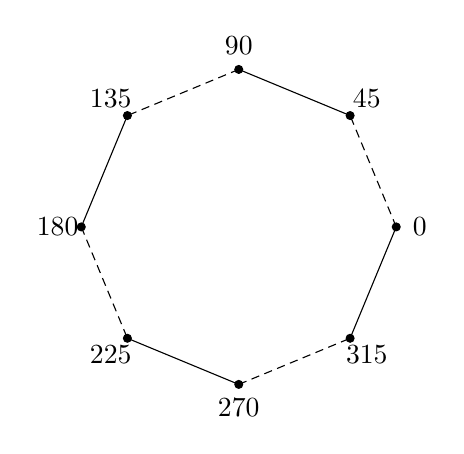
\begin{tikzpicture}
    % Coordinates for the points.
    \foreach\x in {0,45,90,135,180,225,270,315}{%
        \coordinate (\x) at (\x:2);
        \draw[fill=black] (\x) circle (0.05);
        \node at (\x:2.3) {$\x$};
    }

    % Dashed lines for acting by d.
    \draw[densely dashed] (0)   to (45);
    \draw[densely dashed] (90)  to (135);
    \draw[densely dashed] (180) to (225);
    \draw[densely dashed] (270) to (315);

    % Dashed lines for acting by d.
    \draw(45)  to (90);
    \draw(135) to (180);
    \draw(225) to (270);
    \draw(315) to (0);
\end{tikzpicture}
                \caption{Alternate Cayley Diagram for $D_{8}$}
                \label{fig:Alt_Cayley_Diagram_D8}
            \end{figure}
        \end{lexample}